\section*{Vererbung}
	In Java gibt es nur Einfachvererbung, sprich jede Klasse hat maximal eine Basisklasse. Die Subklasse bietet alles was Superklasse bietet und eventuell mehr.\\
	\begin{minipage}[t]{8cm}
		\subsection*{Root Class Object}
		Jede Klasse erbt automatisch (direkt oder indirekt) von der obersten Basisklasse \texttt{Object}. Folgend einige der wichtigsten Methoden der Klasse \texttt{Object}:
		\lstinputlisting{code/Object_Member.java}
		\section*{Typ-Polymorphismus}
		Ein Objekt hat nicht nur den Typ seiner Klasse, sondern auch die Typen seiner Superklassen. Beispiel:
		\begin{minipage}[t]{5cm}
			\lstinputlisting{code/Typ_Polymorphismus.java}
			\vspace*{0.5cm}
			\texttt{@Override}: stellt sicher, dass es die Methode in der Basisklasse gibt
		\end{minipage}
		\hspace*{0.5cm}
		\begin{minipage}[b]{2.3cm}
			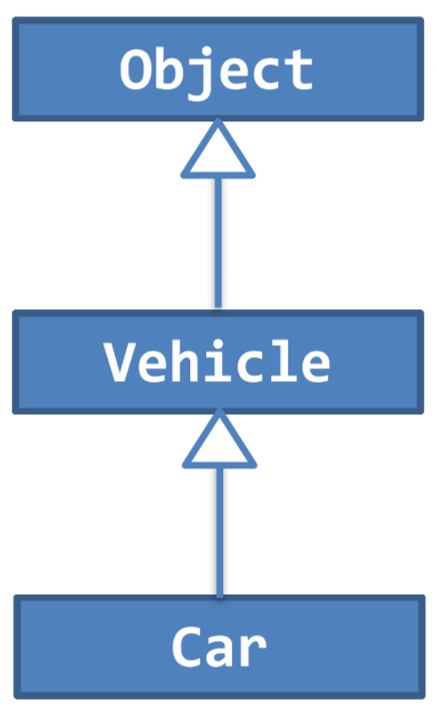
\includegraphics[height=3.8cm, align=t]{pics/Typ_Polymorphismus.PNG}
		\end{minipage}
	\end{minipage}
	\hspace*{0.5cm}
	\begin{minipage}[t]{10.3cm}
		\subsection*{Konstruktor bei Vererbung}
			Das erste Statement in jedem Konstruktor ist der Aufruf des Basis-Konstruktors mittels \texttt{super()}. Dieser wird implizit vom Compiler eingefügt, wenn ein Default-Konstruktor(ohne Parameter) existiert, ansonsten muss er an \textbf{erster} Stelle im Konstruktor explizit aufgerufen werden.
			\lstinputlisting{code/super_Explicit.java}
	\end{minipage}

	
	